\chapter{基于相似微博的流行度预测方法}
\label{chap:three}
\section{引言}
流行度预测在站点优化、广告策划以及市场营销等领域有着重要的应用意义。现有的流行度预测方法主要可以归结为三类:基于特征的有监督学习方法、基于随机过程的方法和基于表示学习的方法。基于特征的方法主要是通过人工提取大量与流行度变化相关的特征,以历史消息的传播数据为样本,学习得到流行度预测函数;基于随机过程的方法则是在生存分析理论的框架下,设计流行度增长过程的强度函数,从而对流行度的到达过程进行建模;基于表示学习的方法则是受深度学习领域的影响,利用深度模型来建模影响流行度变化的因素。这三类方法的详细介绍可参加本论文的第二章。

现有的三类方法在对流行度进行预测时,存在一个共同的缺陷:对历史消息没有进行充分地挖掘和利用。人们对社交网络平台的深度使用,也使得我们积累了大量的历史传播数据。这些历史传播数据中蕴含了丰富的信息,包括消息的不同传播模式信息以及流行度的增长变化信息等,但是现有的方法没有对这部分数据进行充分地利用。基于随机过程的方法通常只是以待预测消息在观测窗口内的转发数据作为输入,而没有显示地利用历史消息;基于有监督学习的方法则是将所有的历史消息作为训练样本,学习得到一个平均的模型。这样的模型没有充分考虑历史数据中不同消息间的差异性以及离群点的影响。因此,本章研究内容的出发点就是设计一种能够充分利用历史数据的流行度预测模型。

近邻思想是机器学习领域的一种重要思想。它的基本出发点是利用样本间的相似性来对样本进行处理,在分类问题和回归问题中都有着重要的应用,例如常用分类问题中常用的$k$--NN模型\citep{keller1985fuzzy}和回归问题中的高斯随机过程方法\citep{williams1996gaussian}都是基于近邻的思想。流行度预测问题同样可以从近邻的角度去考虑。海量的历史传播数据为我们提供了大量的样本。对于待预测的消息,我们可以从海量的历史样本中寻找出与之相近的历史样本,并利用历史样本的流行度变化信息,来对待预测消息的流行度变化进行预测。

 在本章中,我们提出了一种基于相似消息的流行度预测方法。对于待预测的消息,我们根据它在观测窗口内的流行度增长过程,从历史消息中寻找出与之相似的部分消息,再基于相似消息来对该消息后续的流行度变化进行预测。在定义消息之间的相似度时,我们将消息传播中包含的传播模式作为隐变量,利用文本领域的主题模型\citep{blei2003latent}学习得到消息在不同传播模式上的分布来作为消息的表达,进而使用余弦距离来度量消息之间的相似度。我们的方法既充分利用了历史信息,同时也考虑了消息本身传播过程的特异性。在数据集上的实验结果表明,我们的方法在流行度预测任务上要明显优于前两类方法。

\section{相关工作}
流行度预测研究领域的工作非常多,前面提到的基于特征的有监督学习方法、基于随机过程的方法和基于表示学习的方法在第二章中已有详细介绍,这里不再赘述。本节主要介绍一些基于消息间的相似性开展的流行度预测工作。

Kong等人\citep{kong2014predicting}提出了kSAIT模型对为微博平台中消息的转发数进行预测。作者假设同一用户发布的消息在传播过程上是相似的,并在此基础上提出了一种用户特定的转发数预测方法:针对每一个用户,学习得到一个独立的转发数预测函数。作者将用户历史发布的每一条消息在观测窗口内的传播数据中提取出一系列的特征来作为消息的表示。对于用户新发布的消息,作者先计算该消息与用户发布的历史消息之间的相似度,再根据相似度挑选出最高的$k$条历史消息,并根据选取的历史消息来对新发布消息的流行度进行预测。这种方法的先验假设过于理想,并且需要对每一个用户来学习不同的预测函数。此外,在对消息的表示上,需要人工提取特征,并不能真正体现消息在传播过程上的相似性。

基于消息分组思想的流行度预测方法也是对消息间相似度的一种隐式利用。Cao等人\citep{cao2017predicting}在微博数据集上对S--H模型\citep{szabo2010predicting}的适应性进了分析。作者先将所有的训练样本上训练,得到模型的参数;再根据消息在观测窗口的累积流行度,将训练样本分成不同的组别,然后在每个组别上分别训练得到S--H模型的参数。对比两组实验结果,作者发现,不同组别上学习得到的模型参数差异非常大,而且都与全部样本上训练得到的模型间存在着显著的差异。论文中的实验结果表明,`` 将所有的样本作为一个集合进行训练,再将训练得到的模型应用到所有的测试样本上"这样的预测框架在流行度预测问题上存在着明显的缺陷。因此,我们需要对训练样本进行更进一步的挖掘。Hoang等人\citep{hoang2017gpop}则是从用户分组的角度来考虑流行度预测问题。在完成用户分组后,作者也是利用了近邻的思想来对消息进行预测。作者从训练数据中选出与待预测消息相似的$k$条消息,再将这$k+1$条消息的传播数据组成一个三维张量,利用张量填充的方式来对待预测消息的流行度进行估计。
%已有的流行度预测方法大体可以分为两类:基于特征的方法和基于点过程的方法。
%
%基于特征的方法通常将流行度预测问题形式化为回归或分类问题,人工地定义和抽取大量特征,使用有监督的框架来学习特征到流行度之间的变换函数。Szabo等人[11]研究了Digg上的新闻数据和Youtube上的视频数据,发现这些内容早期的流行度和后期流行度之间存在着很强的对数线性相关,并将消息的早期累积流行度为特征,提出了SH(Szabo-Huberman)模型来预测消息的流行度。Pinto等人[12]在SH模型的基础上,将观测窗口内的累积流行度拆分为等长时间间隔内的流行度增长序列,利用多元回归模型来预测流行度。这类工作中,也有研究者专注于分析和发现对流行度预测有指示作用的特征。Suh等人[13]研究了Twitter平台上消息的转发情况,并抽取了一系列的特征来预测消息的最终转发数。实验结果表明,消息中包含的URL和hashtag标签信息,对消息转发数的预测有很重要的指示作用。消息发布者的元信息,包括粉丝数和关注数等,也与最终的预测结果存在很强的关联关系。Bao等人[14]研究了新浪微博上消息转发形成的转发树数据,提取了消息转发树的深度和连接密度两个特征,有效提高了回归模型的预测精度。此外,Cheng等人[15]将流行度预测问题形式化为阶段性的增长预测问题。他们指出,在以往的流行度分类预测问题中,由于流行度本身的分布是幂律的,导致各个类别样本数极度不均匀,从而影响最终的预测效果。因此,他们提出了“kto2k”问题:给定当前流行度为k的消息,预测它们最终的流行度能否增长到2k。 基于样本集中流行度的分布,他们证明了提出的“kto2k”问题是一个均衡的二分类问题,并抽取了内容特征、用户特征、网络结构特征以及时序特征来进行预测。实验结果表明,随着k的增长,分类预测的准确率也在不断提高。
%
%基于点过程的方法通常只利用待预测消息自身的信息,通过对待预测消息在观测窗口内流行度到达过程的建模,来预测消息后续流行度的变化。这类方法将流行度的增长过程形式化为一个计数过程[16](Counting process),并将强度函数(Intensity function)的刻画作为模型的核心。强度函数 刻画了给定历史信息 下,在时间窗口 内有新事件发生的概率,即:
% 。
%基于这一框架,Shen等人[3]提出了基于自增强泊松过程(Reinforced Poisson process, RPP)的RPP模型。在建模消息的强度函数时,考虑了消息本身的吸引力、时间衰减机制和富者愈富机制。Gao等人[4]将RPP模型应用到新浪微博中,并对几种机制的作用形式进行了修正。Bao等人[5]采用了自激励Hawkes过程(Self-exciting Hawkes process)来建模强度函数,刻画了消息传播过程中转发用户带来的激励作用。Zhao等人[17]在自激励过程的基础上,进一步引入了用户的影响力信息。他们将用户的粉丝数加入到强度函数的建模中,进一步提升了模型的预测效果。这类方法由于没有利用其他历史消息的信息,预测能力比较有限。
%
%此外,Mishra等人[18]提出了将上述两类方法融合的方法。他们先利用自激励过程来建模消息在观测窗口内的流行度增长过程,再将学习得到的参数与人工抽取的其他过程合并,利用回归模型来预测消息的最终流行度。近年来,深度学习的方法在流行度预测领域也取得了不错的的进展。Li等人[19] 提出了端到端的DeepCas模型。他们在监督学习框架下,先利用深度学习模型将消息在观测窗口内的转发情况表示为向量,再利用神经网络模型学习消息的流行度增长与转发向量间的转换函数。Cao等人[20]在自激励过程的启发下,提出了DeepHawkes模型。他们利用深度学习模型,刻画了传播过程中的用户影响力、用户激励以及时间衰减效应等影响因子,在数据集上取得了很好的预测效果。

\section{模型}
\subsection{问题形式化}
消息$i$在给定时间窗口$[0,T]$内的传播数据可以用时间戳序列$C^i=\{t_k^i|t_k^i<T,k=1,2,...,n_i\}$表示,其中$n_i$表示消息$i$在时间窗口内的转发次数,$t_k^i$表示第$k$次转发距离消息源发时间的间隔。给定一组历史消息在完整窗口$[0,T]$的传播数据和一组待预测消息在观测窗口 $[0,T_0]$($T_0<T$)的传播数据,我们需要对待预测消息在时间窗口$[T_0,T]$内的流行度变化进行预测。

\subsection{整体预测框架}
不同于传统的基于特征的方法和基于点过程的方法,我们提出了一种基于相似消息的流行度预测方法。我们对所有消息在观测窗口的传播数据进行表示,对于待预测的每一条消息$j$ ,我们在历史消息中找到与之相似的$K$条消息,利用这$K$条消息在窗口$[T_0,T]$内的数据,来预测消息$j$在预测窗口$[T_0,T]$内的流行度。我们提出的方法,既充分利用了历史消息的传播数据,同时又避免了对所有的消息使用统一的预测模型,充分考虑了消息传播过程的特异性。在我们的模型中,如何对消息的传播数据进行表示,进而找到与之相似的历史消息,是至关重要的部分。

\subsection{消息传播数据的表示}
时间序列$(x_1,x_2,...,x_N)$通常被用来将消息的传播数据转化为定长的向量化表示,其中 $N$表示划分的等长时间区间的个数,$x_i$表示在第$i$个时间间隔内流行度的增长量。这种时间序列的表示方式能一定程度上反应消息的流行度变化趋势,但是这种表示方法的效果受时间区间粒度的影响,同一条消息在不同大小的时间区间下的表示差异较大。另外,它也不能刻画消息在传播模式上的区别。事实上,消息的传播过程中包含着不同的传播模式,如快速爆发的模式、均匀增长的模式、逐渐衰退的模式等。图\ref{fig:example}中展示了两条示例消息的传播过程。从图中可以看到,在时间序列表示下,以5个单位时间为一个时间区间,两条消息的表达都是$(25,21)$,但是两条消息的传播过程并不相同。第一条消息经历了平稳增长和衰落的过程,可以预见后续的流行度增长量会比较小;而第二条消息在经历了第1个时间间隔内的快速增长和衰落后,在第2个时间间隔内又迎来了平稳增长的过程,后续的流行度应该会持续增加。因此,基于时间序列的表示方法,会忽略消息传播过程所包含的不同传播模式,难以真正捕获传播过程相似的消息用于预测。
\begin{figure}[!htbp]
  \centering
  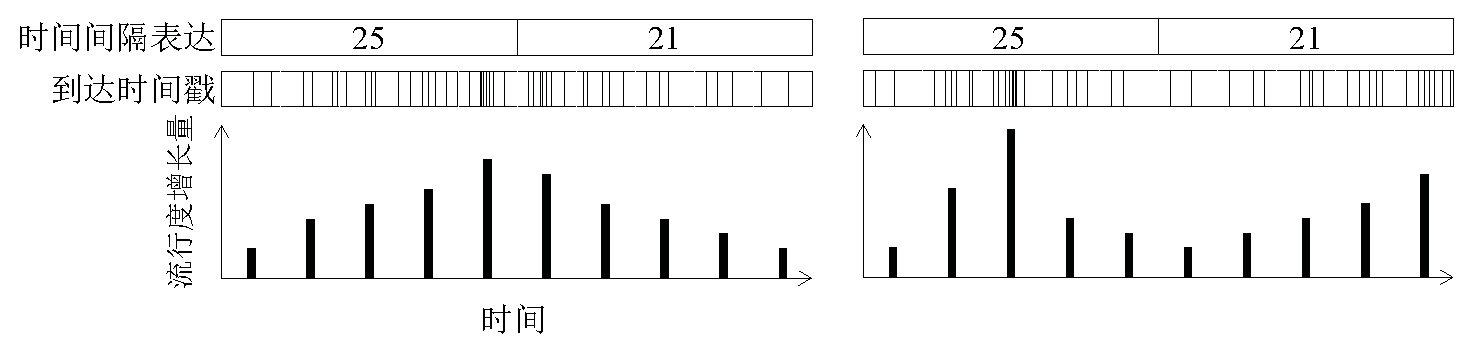
\includegraphics[width=1\textwidth]{3-example}
  \caption{两条示例消息的传播数据}
  \label{fig:example}
\end{figure}

进一步地观察图\ref{fig:example},我们可以发现:消息在处于不同的传播模式时,转发到达的速率不同,形成的转发时间间隔的分布也不相同。当消息处于快速爆发的模式时,会产生大量的短时间间隔;而当消息处于衰退模式时,会产生较少但是持续时间长的转发时间间隔。因此,消息在传播过程中产生的时间间隔数据,可以帮助推断消息所处的传播模式。
我们将消息的传播过程类比于文档的产生过程,利用文档主题模型来学习消息传播数据的表示。我们将消息的传播模式类比于文档的主题,消息转发过程中产生的时间间隔类比于文档中的词。每个消息的传播数据可以表示为在不同传播模式上的分布。我们统计了数据集中转发时间间隔的分布,结果如图\ref{fig:intervalDist}所示。从图中可以发现,转发时间间隔的分布与文档集中词的分布是类似的,都服从幂律分布。
\begin{figure}[!htbp]
  \centering
  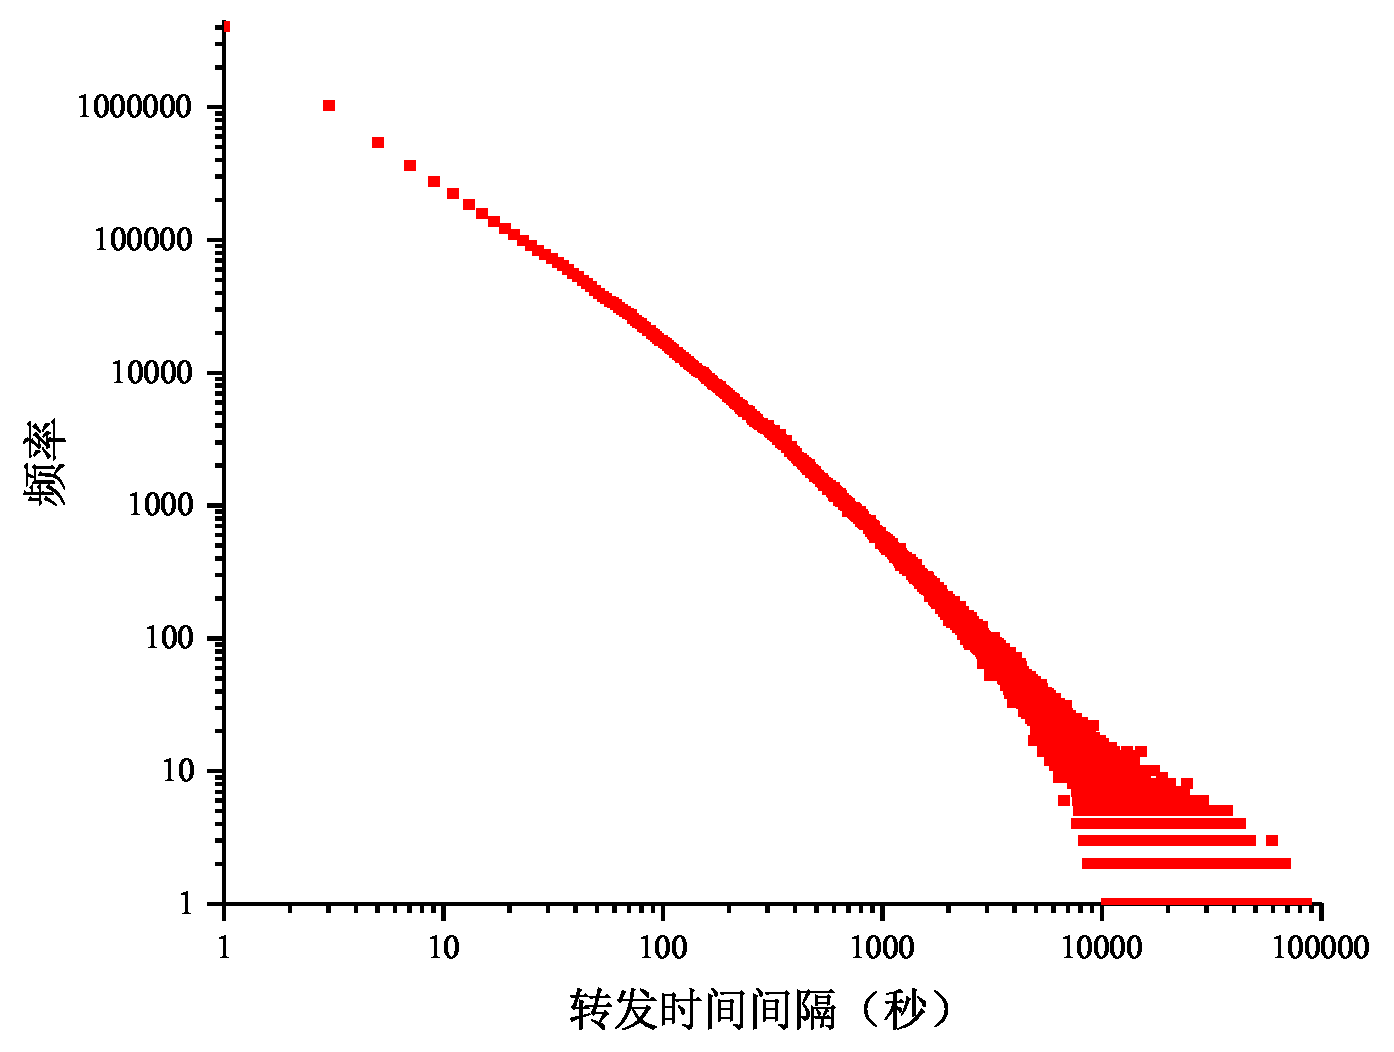
\includegraphics[width=0.8\textwidth]{3-IntervalDist}
  \caption{数据集中消息转发时间间隔的分布}
  \label{fig:intervalDist}
\end{figure}

对于一条消息$i$,它的第$k$个转发时间间隔$\Delta t_k^i$定义为$\Delta t_k^i=t_k^i-t_{k-1}^i$。 类似于LDA模型,我们采用如下的产生过程来生成$\Delta t_k^i$:
\begin{itemize}
\item	消息$i$根据自身传播模式的分布,采样一个传播模式$P$;
\item	根据传播模式$P$下产生时间间隔的分布,采样得到$\Delta t_k^i$。
\end{itemize}

我们采用了LDA模型来从时间间隔数据中学习得到消息传播模式的分布,将其作为消息的表示。在模型学习时,我们将消息在观测窗口$[0,T_0]$内的数据$C^i=\{t_k^i|t_k^i<T,k=1,2,...,n_i\}$转成时间间隔 $\{\Delta t_k^i|\Delta t_k^i=t_k^i-t_{k-1}^i,k=1,2,...,n_i\}$。每条消息的时间间隔数据作为一个文档,所有训练数据集中出现过的时间间隔的集合作为词汇表。另外,我们方法使用了绝对的时间间隔数据,避免了时间序列表示方法中时间区间粒度的问题。

\subsection{消息流行度预测}
在学习得到消息的表示之后,我们提出了一种基于相似消息的流行度预测方法。对于每一条待预测消息$j$,我们首先利用训练集上学习得到的LDA模型,推断它在不同传播模式下的分布作为它的表示,然后计算它与训练集中所有历史消息的相似程度,选取出相似度最高的$K$条历史消息。对于每个待预测的时间点,我们将抽取的$K$条历史消息在该时间点的流行度求取平均值,作为消息$j$在该时间点的流行度的预测。为了避免离群点对预测结果的影响,我们使用截尾均值[21](Trimmed mean)作为平均值的计算方式。截尾均值的定义为:在计算序列$\{s_1,s_2,...,s_N\}$的截尾均值时,先将该序列按照从小到大的顺序排列,得到$\{\widetilde{s_1},\widetilde{s_2},...,\widetilde{s_N}\}$;再去掉序列中最大的$\varepsilon$\%数据和最小的$\varepsilon$\%数据,将剩余数据的均值作为序列的截尾均值。其中$\varepsilon$是待设置的参数。

我们模型的整体预测框架如图\ref{fig:architecture} 所示。
\begin{figure}[!htbp]
  \centering
  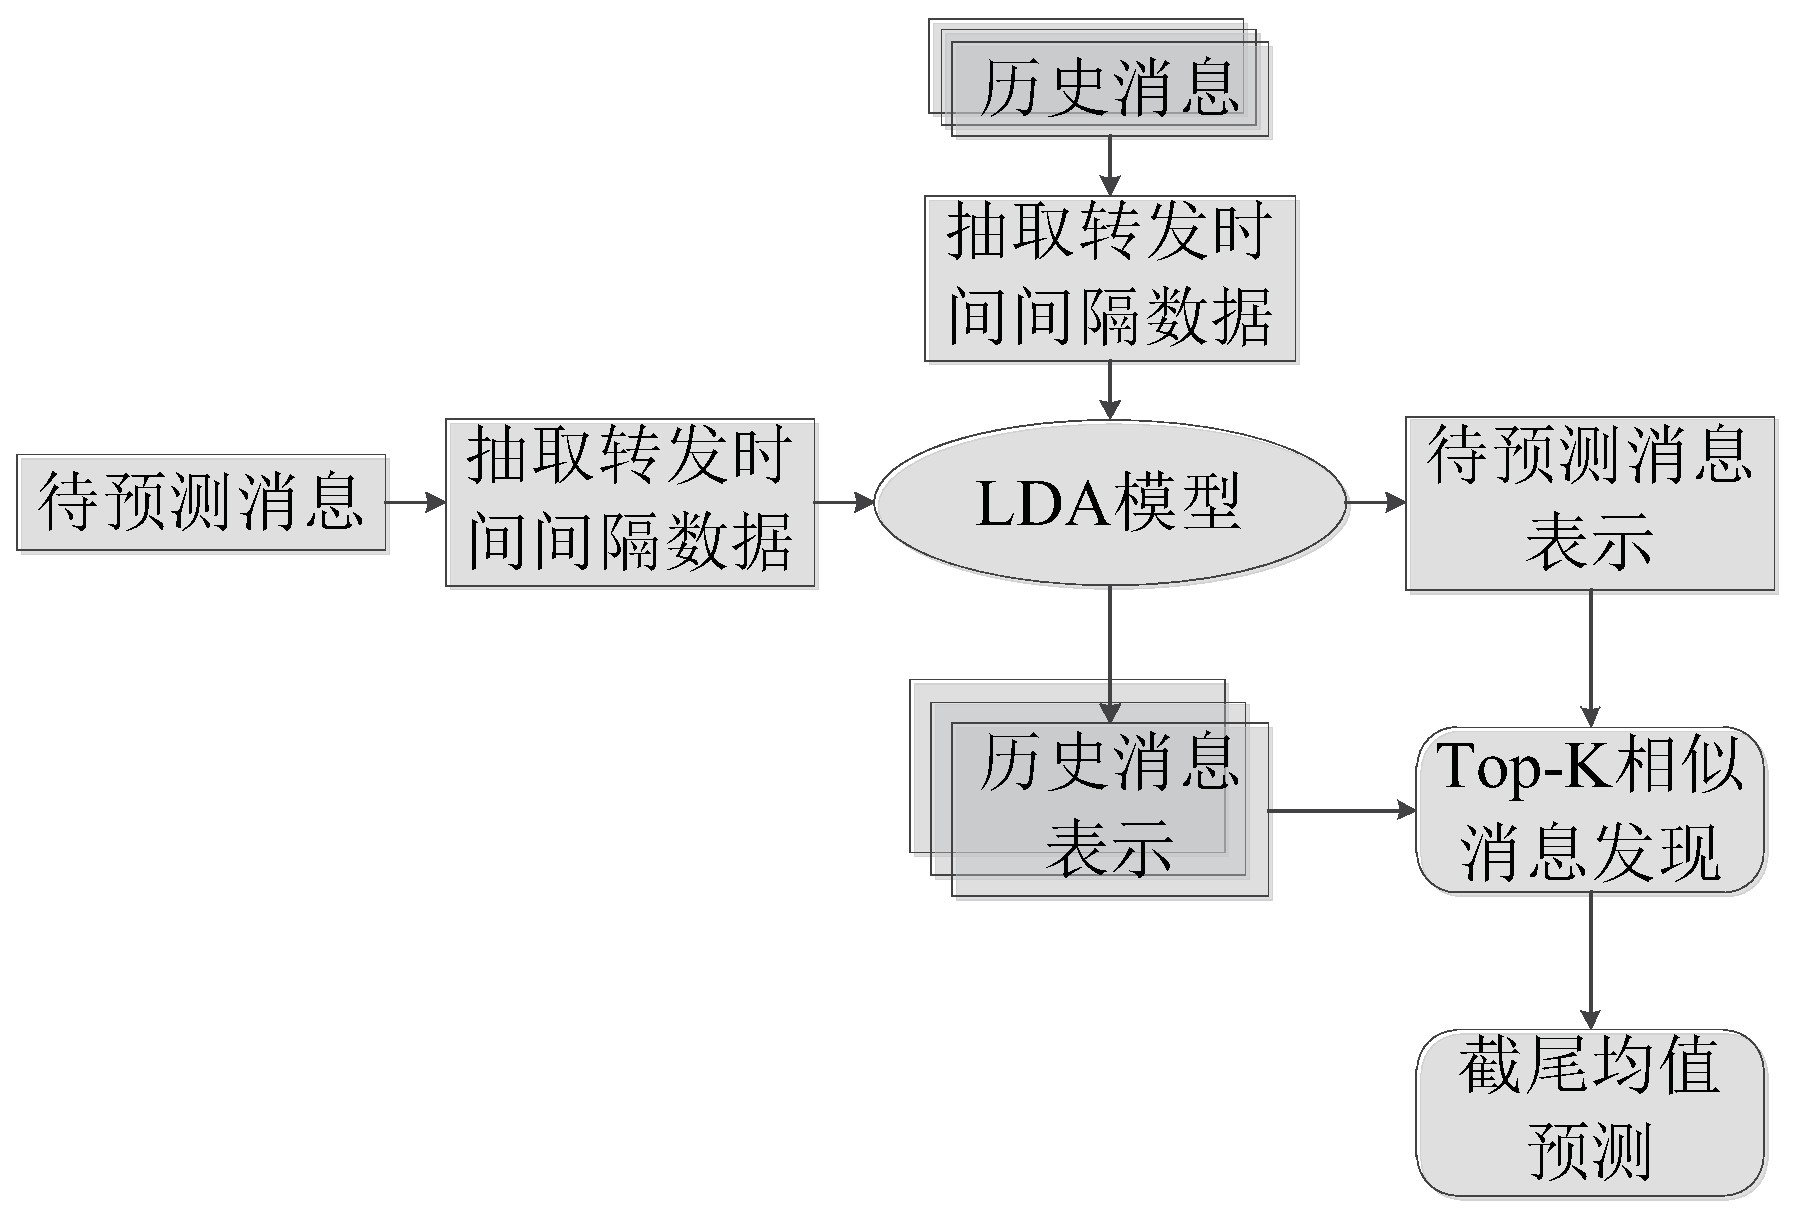
\includegraphics[width=0.8\textwidth]{3-architecture}
  \caption{模型的整体预测框架}
  \label{fig:architecture}
\end{figure}

\section{实验}
\subsection{实验数据}
我们抓取了微博上某一天的全部源发消息和它们发布后24小时内的转发数据来作为我们的实验数据。我们过滤了发布1小时后累计转发数小于10的消息,最终用于实验的数据集包含了6.5万条源发消息和它们在发布后24 小时内的转发数据。我们统计了数据集中微博的流行度分布,结果如图\ref{fig:retweetDist}所示。
\begin{figure}[!htbp]
  \centering
  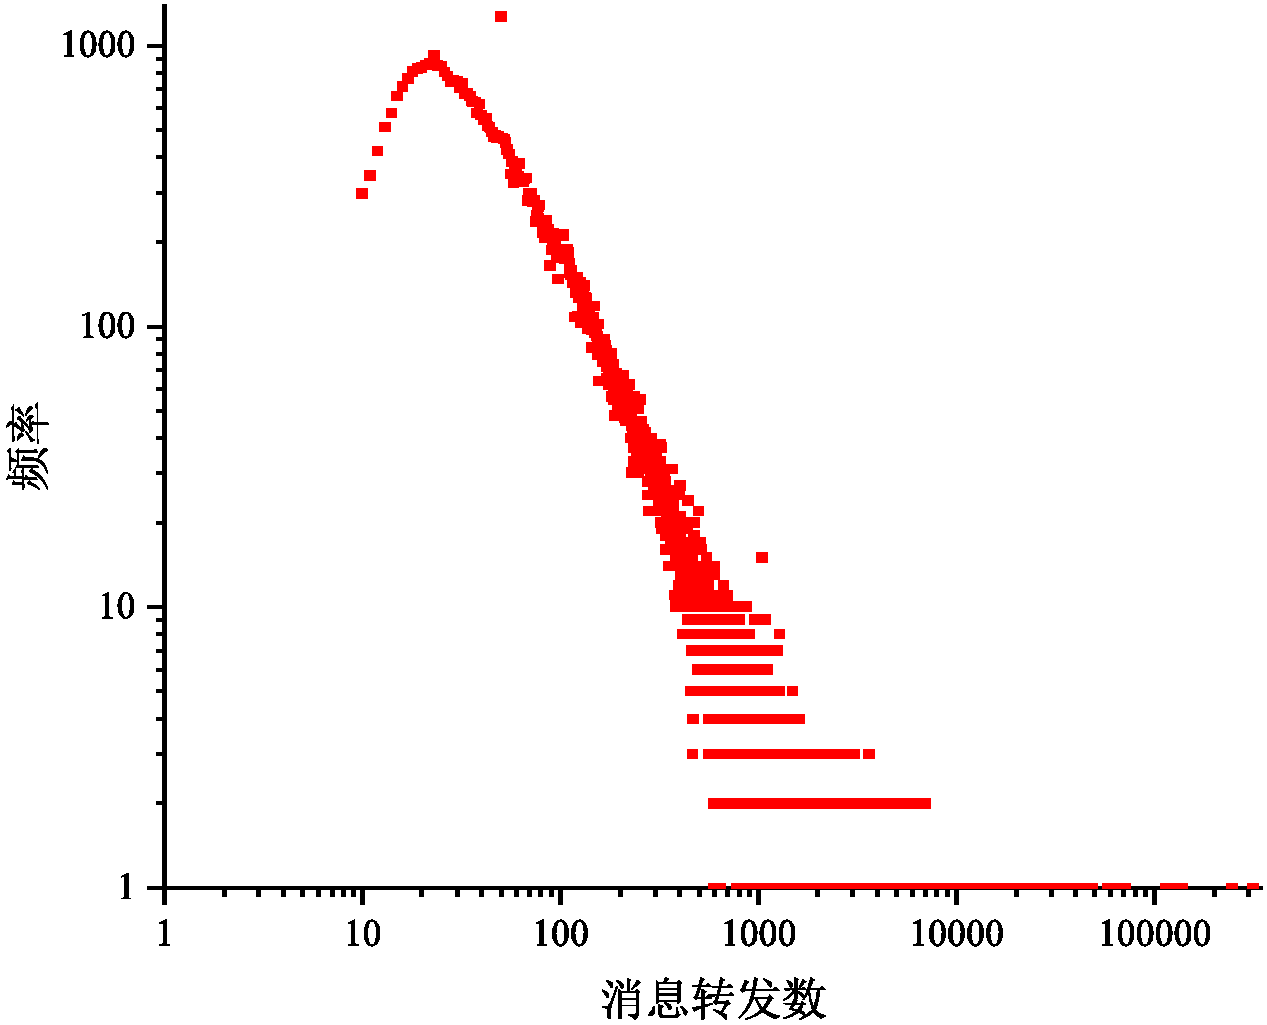
\includegraphics[width=0.8\textwidth]{3-RetweetDist}
  \caption{数据集中消息流行度的分布}
  \label{fig:retweetDist}
\end{figure}

我们将数据集平均分成5 份,轮流选取其中1 份为测试集,剩余4 份为训练集来进行实验。所有展示的实验结果均为5 个测试集的平均结果。
\subsection{实验准备}
\subsubsection{对比模型}
我们选取了以下三个模型来和我们的模型进行对比:
\begin{itemize}
\item 	RPP模型\citep{shen2014modeling}:采用了自增强泊松过程来刻画流行度的到达过程,考虑了消息自己的吸引力、时间衰减效应和富者愈富效应;
\item 	Pinto模型\citep{pinto2013using}:将消息在观测时间窗口内的转发数据表示为时间序列,利用多元线性回归模型来学习时间序列特征与流行度之间的变换函数;
\item SeqSim模型:和我们提出的模型一样,SeqSim 模型也是先从历史消息中寻找到和待预测消息相似的消息,再利用相似消息进行预测。不同于我们的模型,SeqSim模型直接使用时间序列来表示消息的传播数据。
\end{itemize}
\subsubsection{评价指标}
我们使用了平均绝对百分误差(Mean Absolute Percentage Error, MAPE)来度量不同模型的预测效果。模型在预测时间点$t$的MAPE值定义如下:
 \begin{displaymath}
 MAPE(t)=\frac{1}{m}\sum_{i} |\frac{r^i (t)-\widetilde{r^i (t)}}{r^i (t)}|\text{。}
 \end{displaymath}
其中,$m$是测试集的大小,$r^i (t)$表示$t$时刻消息$i$的真实流行度,$\widetilde{r^i (t)}$表示模型对消息$i$在$t$时刻的流行度的预测。MAPE的值越低,表示模型的预测效果越好。
\subsubsection{参数设置}
在我们的实验中,消息的观测窗口设置为1小时,预测窗口设置为24小时。在利用LDA模型学习消息的表示时,LDA的主题数为4时,效果最好,因此实验部分的结果均为主题数为4时的结果。主题数对预测效果的影响将在实验分析章节中进行讨论。在选取最相似的历史消息时,我们将$K$设置为10,即为每条待预测消息找到与之最相似的10条历史消息来进行预测。对于Pinto 模型和SeqSim模型,在生成时间序列时,我们选择的时间区间的长度为5分钟。在使用截尾均值进行预测时,截尾均值的参数$\varepsilon$\%设置为10\%。
\subsection{实验结果}
我们以消息发布后1小时内的转发情况作为观测,来预测后续每隔1小时后消息的流行度情况,实验结果如图\ref{fig:exprResult}所示。
\begin{figure}[!htbp]
  \centering
  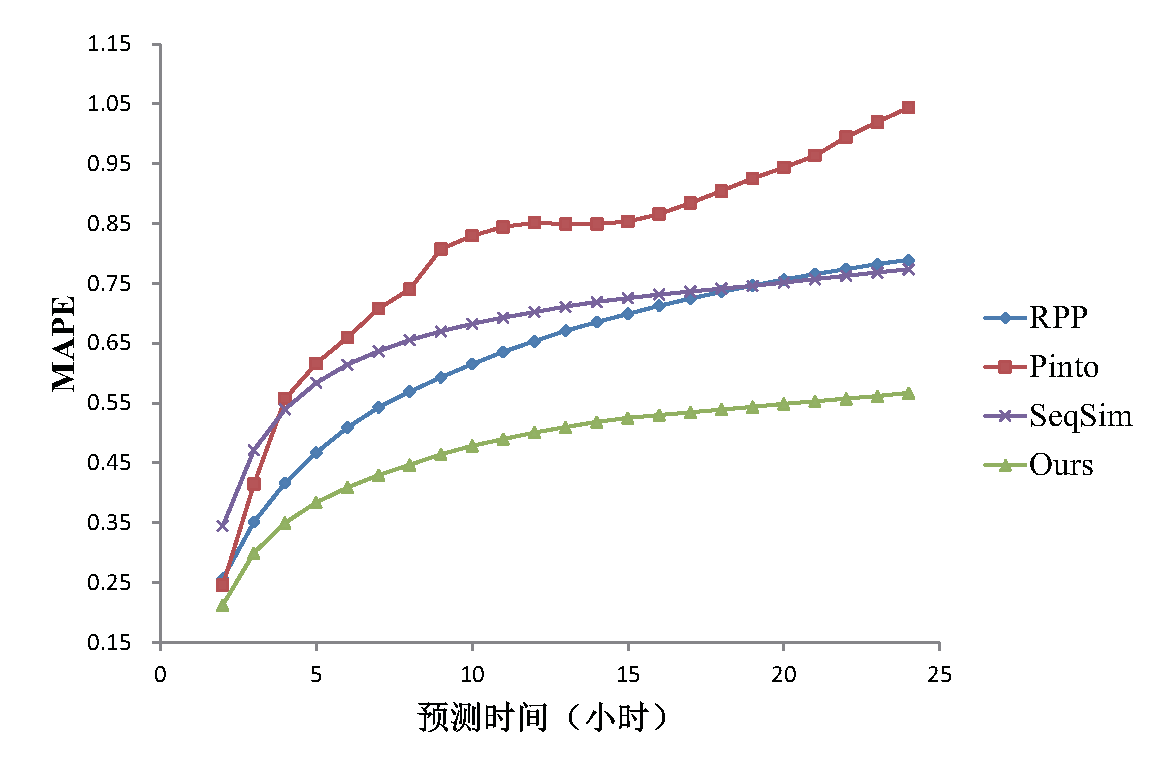
\includegraphics[width=0.8\textwidth]{3-expr}
  \caption{不同模型的流行度预测效果}
  \label{fig:exprResult}
\end{figure}


从图\ref{fig:exprResult}中可以看出,我们提出的模型的预测效果要明显优于其他3个模型。Pinto模型的表现效果最差,因为它用一个模型来预测所有的待预测消息,噪音影响很大。比较Pinto模型和SeqSim模型可以看出,利用相似微博来预测流行度,可以有效地区分出消息本身的特异性,从而显著地提升预测效果。对比SeqSim模型和我们提出的模型的结果可以看出,相比于时间序列的表示方法,我们的提出的基于消息传播模式的表示方法,可以更好地刻画消息的传播过程,进而找到传播过程相似的历史消息来进行预测,得到更精确的预测效果。另外,综合对比两个基于相似消息的模型和其他两个模型,可以发现基于相似消息的模型在进行预测时,随着时间的增长,预测误差的增长更加平稳,预测性能更好。
\subsection{实验分析}
\subsubsection{LDA模型中主题个数的影响}
在利用LDA模型进行表示学习时,主题个数是一个非常重要的超参。我们对不同主题个数设
定下的预测效果进行了实验,结果如图\ref{fig:ldaTopic}所示,其中 表示主题个数, 表示预测时刻。
从图\ref{fig:ldaTopic}可以看出,在不同的预测时间点上,主题个数为4 的模型的预测效果都要明显地由于其他模型,因此,在对比实验中,我们将LDA模型的主题个数设置为4。
\begin{figure}[!htbp]
  \centering
  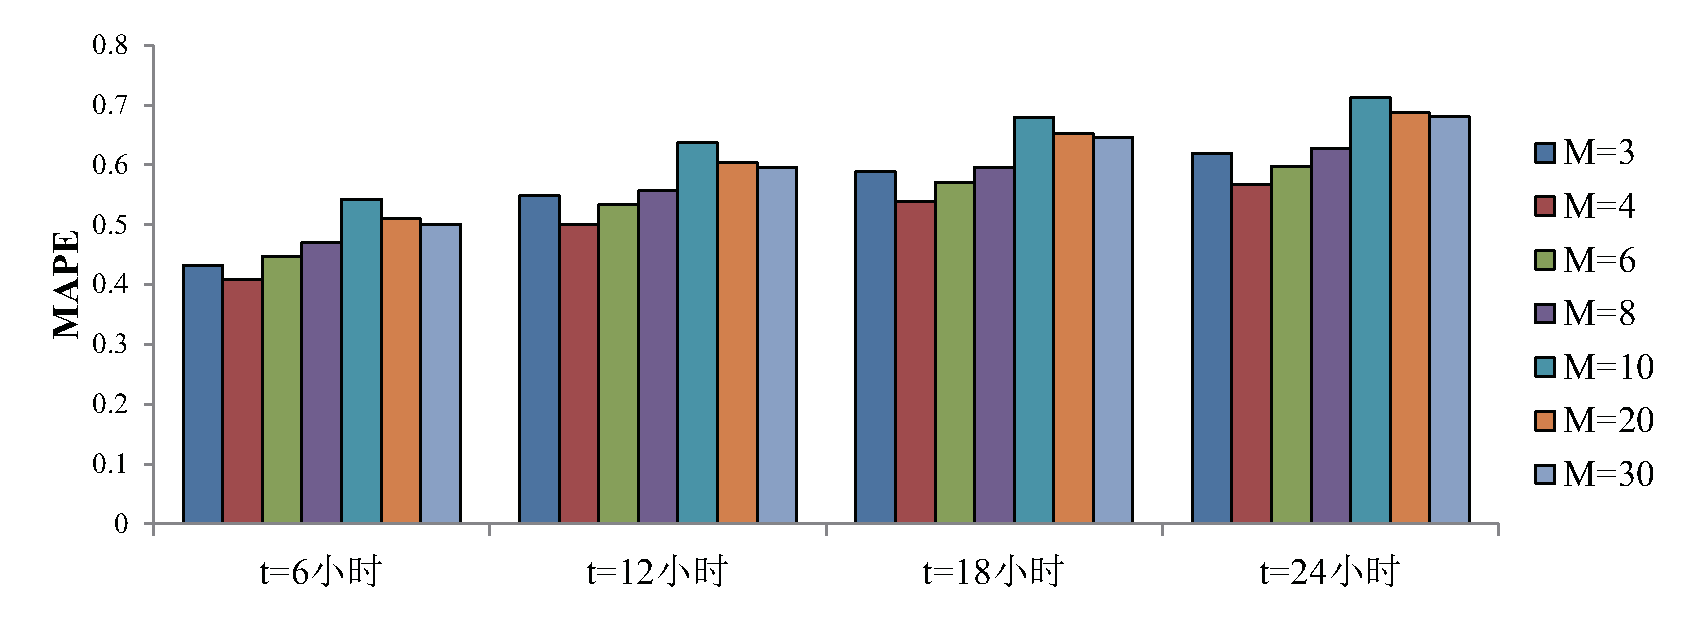
\includegraphics[width=1\textwidth]{3-LDATopic}
  \caption{不同主题数目下模型的预测效果}
  \label{fig:ldaTopic}
\end{figure}

\subsubsection{相似消息分析}
我们在图\ref{fig:simExample}中展示了部分待预测消息以及模型找到与之相似的历史消息的传播数据。图中竖线标识的位置为观测窗口的大小,红点数据标识了待预测消息的流行度变化情况。从图中可以看到,我们找到的相似消息,在观测窗口内的传播过程和流行度大小与待预测消息非常相似;同时在预测时间窗口中,消息的流行度变化趋势也非常一致。这表明我们提出的基于传播模式的表示方法,可以有效地刻画消息的传播过程,从而找到那些变化趋势相近的历史消息来辅助预测。另外,从图中可以看出,找到的近似消息中存在离群点,这也说明了采用截尾平均值的必要性。
\begin{figure}[!htbp]
  \centering
  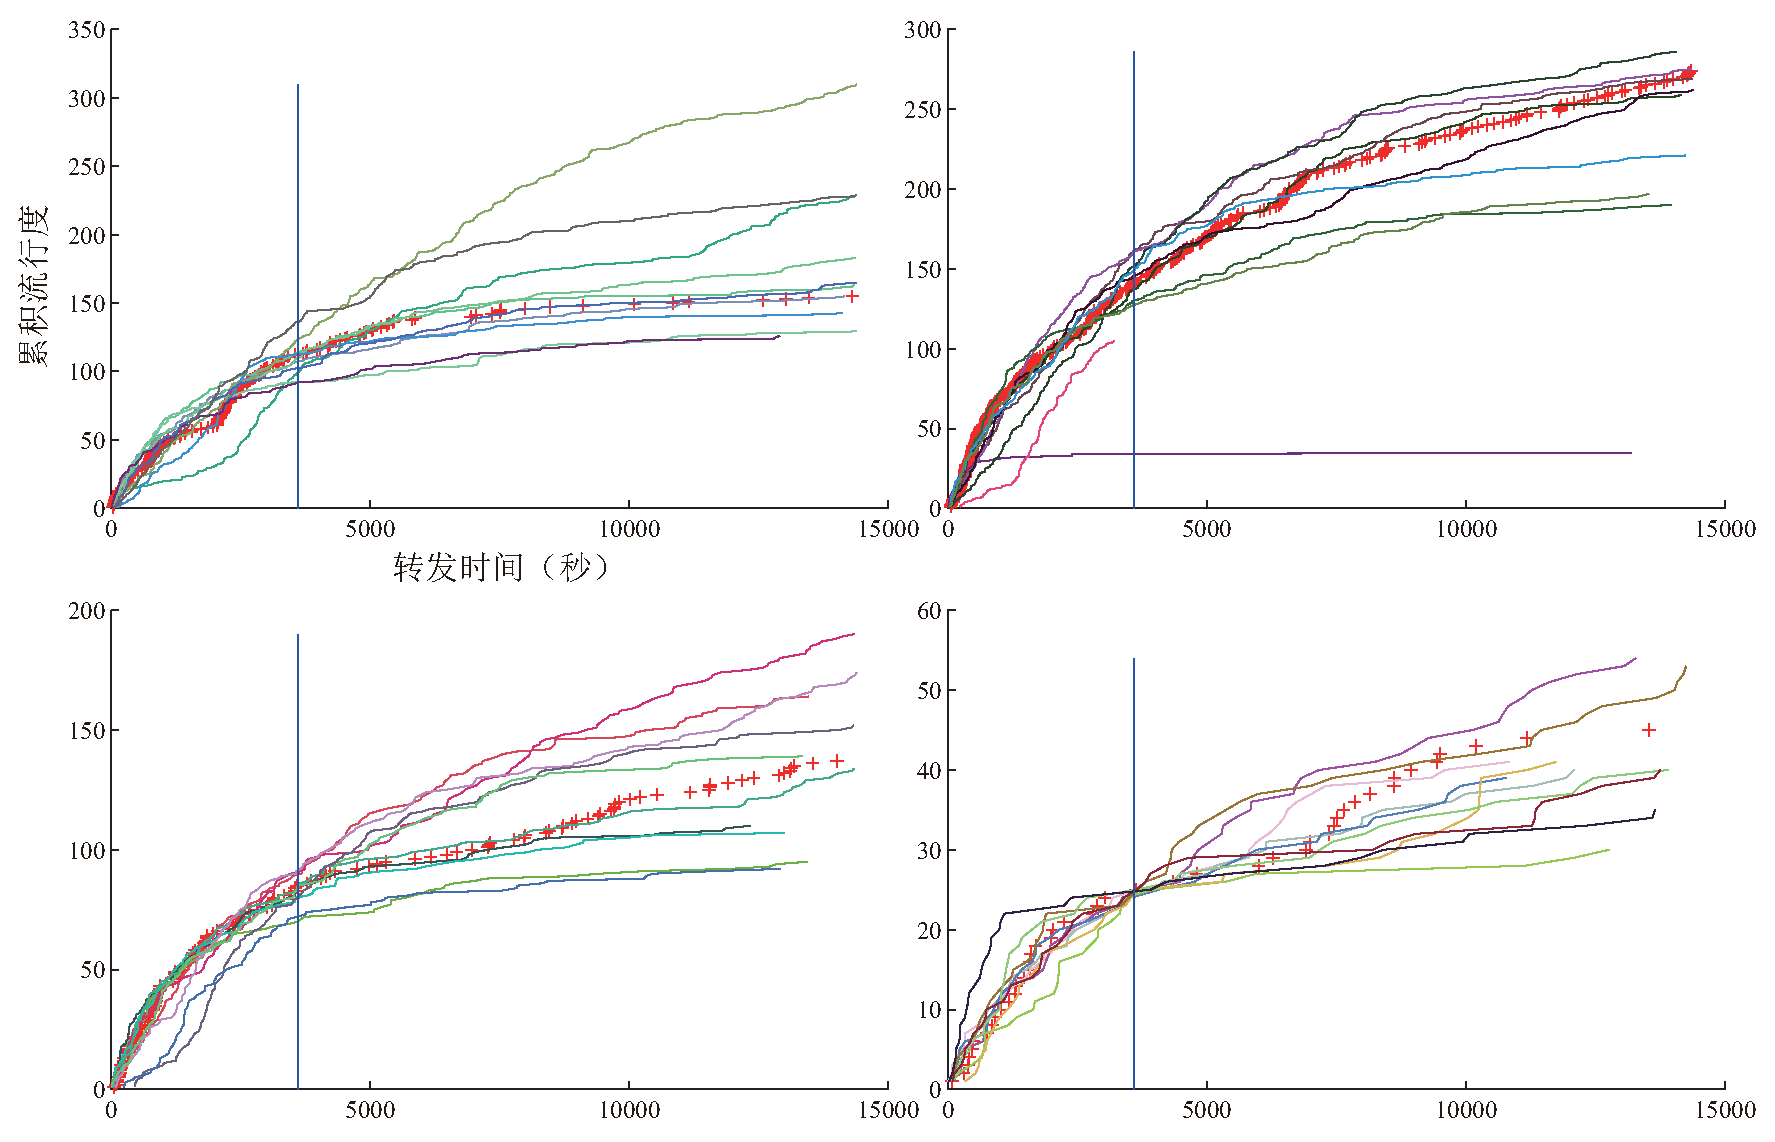
\includegraphics[width=1\textwidth]{3-SimSample}
  \caption{待预测消息及相似微博示例}
  \label{fig:simExample}
\end{figure}

\section{本章小结}
针对现有的两类流行度预测方法的不足,本章中提出了一种基于相似消息的流行度预测方法。对于每一条待预测的消息,我们从历史消息中选取出传播相似度最高的K条消息来进行预测。在计算消息间的相似度时,我们利用了文档主题建模领域的LDA模型,来学习得到消息的表示。我们将消息转发过程中产生的时间间隔数据作为输入,将消息中包含的不同的传播模式作为隐变量,利用LDA模型,学习得到消息在不同传播模式上的分布作为消息的表示。数据集上的实验结果表明,我们的方法能够有效地发现传播模式相近的消息,进而取得了更好的流行度预测效果。
